\chapter{Introduction} 

Discrete event simulation (DES) is a computational methodology for
modeling and analysis of a wide spectrum of systems.  In DES, the
system being modeled is logically subdivided into small, independent
but interacting entities with their own independent states.  The
model and implementation of an entity is called a Logical Process
(LP) which manage the state assocated with them.  Accordingly, a DES
is essentially designed as a set of logical processes (LPs) that
interact with each other.  LPs interact by exchanging and processing
discrete-timestamped events or messages~\cite{jafer-13}.  Processing
an event essentially introduces a change in an LP's state and causes
the LP to generate additional events to itself or other LPs in the
model.

A key aspect of DES is that state changes occur at discrete
times~\cite{fishman-13}.  At each point in time in a simulation, a
virtual time-stamp is assigned to an event and the event precipitates
a transition from one state to another state. This change in system
state is used to represent the dynamic nature and behavior of a
real-world system~\cite{fujimoto-90}.

DES has been used in a variety of fields in academia, industry and the
public sector as a tool to help inform knowledge and to improve
decision-making processes~\cite{fishman-13}. DES provides an effective
means for analyzing real or artificial systems without the constraint
of limited resources such as time, financial costs, or safety. For
example, the simulation of a battlefield environment can deliver
insightful information to military planners on enemy troop movements,
tactics and capabilities during strategic planning
efforts~\cite{hill-01}. A discrete event simulation of the battlefield
allows military leaders to examine the impacts of decisions without
the real-world risks associated with committing forces to dangerous
environments.

\section{Parallel Simulation}

Parallelism in computing frameworks that support DES increase
performance throughput that is needed to construct and execute large
scale and complex simulation models. With the growth and prevalence of
semiconductor technology, cheaper and powerful multi-processors can be
instrumented to achieve greater computing power for parallel discrete
event simulations (PDES).  In parallel simulations, LPs are subdivided
or partitioned to operate on different compute units.  However, event
processing on the different compute units must be synchronized to
ensure causally consistent event processing.  Consequently, the
speedup achieved using multi-core and multi-processor systems requires
efficient strategies to minimize synchronization costs.

Currently, two broad types of synchronization methods are used in
PDES, namely: conservative and optimistic approaches~\cite{jafer-13}.
Conservative methods tightly coordinate event processing so that
causal violations do not occur.  Optimistic methods, such as Time
Warp~\cite{jafer-13}, loosely synchronize LPs -- they permit temporary
causal violations to occur but detect and recover from causal
violations.  Recently, optimistic synchronization method have shown to
outperform conservative methods for certain classes of
systems~\cite{jafer-13}.


\section{Managing Pending Events}

Sequential and parallel DES are designed as a set of logical processes
(LPs) that interact with each other by exchanging and processing
timestamped events or messages~\cite{jafer-13}. Events that are yet to
be processed are called "pending events". Pending events must be
processed by LPs in priority order to maintain causality, with event
priorities being determined by their timestamps. Consequently, data
structures for managing and prioritizing pending events play a
critical role in ensuring efficient sequential and parallel
simulations~\cite{jones-86,ronngren-97,brown-88,franceschini-15}. The
effectiveness of data structures for event management is a conspicuous
issue in larger simulations, where thousands or millions of events can
be pending~\cite{carothers-2010,yeom-14}. Large pending event sets can
arise when a model has many LPs or when each LP generates / processes
many events. Overheads in managing pending events is magnified in fine
grained simulations where the time taken to process an event is very
short. Furthermore, the synchronization strategy used in Time Warp (an
optimistic synchronization strategy) can further impact the
effectiveness of the data structure due to additional processing
required during rollback-based recovery operations.

\section{Thesis Statement}

This research proposes and explorers multi-tier data structures for
the improved management of the pending event set in sequential and
optimistic parallel simulations.  The objective of the research is to
develop and assess effectiveness of novel data structures for managing
pending events.  Specifically, this thesis proposes multi-tiered data
structures called 2-tier Ladder Queue (2tLadderQ) and 3-tier Heap
(3tHeap) for managing pending events.  Experimental assessment of the
proposed data structures has been conducted by comparing their
effectiveness using benchmark simulations and a fine-tuned version of
the Ladder Queue~\cite{tang-05}.  The Ladder Queue, with amortized
O(1) time complexity, has been used for comparison because it has
shown to to be very efficient for sequential DES. \newline

\textbf{Thesis:} multi-tiered data structures, especially the novel,
\textbf{2tLadderQ} and \textbf{3tHeap} pending event structures
outperform all other data structures in sequential and optimistic
parallel simulations.

\chapter{Related Works}

Many investigations have explored the effectiveness of a wide variety
of data structures for managing the pending event set in sequential
and parallel discrete event simulation (PDES).  The prior
investigations in PDES area fall under two broad categorizes, namely:
shared memory versus distributed memory data structures.  Shared
memory data structures focus on managing pending events in PDES that
use multiple threads for parallelism.  Such simulations are typically
performed on large shared memory machines with many-core CPUs or
dedicated GPGPUs or coprocessors.  These data structures focus on
enabling concurrent access to add or remove pending events from
multiple threads while avoiding race conditions.  Race conditions are
voided using conventional lock-based approaches such as semaphores or
mutexes.  Recently, lock-free data structures based on special
check-and-set (CAS) instructions have also been proposed to enable
efficient, thread-safe, and concurrent access.

Distributed memory data structures focus on enabling efficient
single-threaded operation.  However, these data structures need to
enable managing events reveived over communication channels from other
remote processes involved in PDES.  This thesis focuses on sequential
simulations as well as distributed memory PDES based on Time Warp
synchronization.  Accordingly, this chapter focuses on closely related
work in sequential and distributed memory PDES.

Dickman~\cite{dickman-13} compare event list data structures that
consisted of Splay Tree, STL Multiset and Ladder Queue. However, the
focus of their paper was in developing a framework for handling
pending event set data structure in shared memory PDES. A central
component of their study was the identification of an appropriate data
structure and design for the shared pending event
set. Gupta~\cite{gupta-14} extended their implementation of Ladder
Queue for shared memory Time Warp based simulation environment, so
that it supports lock-free access to events in the shared pending
event set. The modification involved the use of an unsorted lock-free
queue in the underlying Ladder Queue
structure. Marotta~\cite{marotta-16} contributed to the study of
pending event set data structures in threaded PDES through the design
of the Non-Blocking Priority Queue (NBPQ) data structure. A pending
event set data structure that is closely related to Calendar Queues
with constant time performance.

Recently, Franceschini~\cite{franceschini-15} compared several
priority-queue based pending event data structures to evaluate their
performance in the context of sequential DEVS simulations. They found
that Ladder Queue outperformed every other priority queue based
pending event data structure such as Sorted List, Minimal List, Binary
Heap, Splay Tree, and Calendar Queue. Tang~\cite{tang-05} and
Franceschini~\cite{franceschini-15} both use the classic Hold
benchmark simulation model used in this research.

\section{Ladder Queue (ladderQ)} 

The Ladder Queue (ladderQ) is a priority queue implementation proposed
by Tang et al~\cite{tang-05} with amortized constant time complexity.
Several investigators have independently verified that for sequential
DES the \textbf{ladderQ} outperforms other priority queues, including:
simple sorted list, binary heap, Splay tree, Calendar queue, and other
multi-list data
structures~\cite{dickman-13,franceschini-15,tang-05}. There are two
key ideas underlying the Ladder Queue, namely: minimize the number of
events to be sorted and delay sorting of events as much as possible.
However, in contrast to the \textbf{ladderQ}, the other data
structures always fix-up and maintain a minimum heap property.

As shown in Figure~\ref{fig:ladderQ}(a), the ladder queue consists of
the following 3 substructures:

\begin{enumerate}[leftmargin=*,topsep=0pt]

\item \emph{Top}: An unsorted list which contains events scheduled
  into the distant future or epoch.

\item \emph{Ladder}: Consists of multiple rungs, \textit{i.e.,} list
  of buckets. Each bucket contains list of events with a finite range
  of time stamp values. Hence, although events within a bucket are not
  sorted, the buckets on a rung are organized in a sorted order. The
  \textbf{ladderQ} minimizes the number of events to be finally sorted
  by recursively breaking large buckets into smaller buckets in lower
  rungs of its ladder. Lower rungs in the ladder have smaller buckets
  with smaller time ranges and the maximum number of rungs in Ladder
  is 8.

\item \emph{Bottom}: This substructure contains a sorted list of
  events to be processed. Inserts into \emph{Bottom} must preserve
  sorted order. Hence, the \textbf{ladderQ} strives to maintain a
  short bottom by moving events back into the ladder, as needed. The
  default threshold value at which events from Bottom are moved into
  Ladder is 50~\cite{tang-05}.

\end{enumerate}

At the beginning of a simulation, enqueue operations only involve the
insertion of events into \emph{Top}. As the simulation progresses, the
insertion of events can occur at any level of the data structure. The
insertion of events in \emph{Top} and Ladder is an O(1) operation that
involves appending events to a list that remains unsorted. The onset
of dequeue operations involves moving unsorted events from \emph{Top}
into a newly formed rung in Ladder. The time range or bucket-width of
a rung is established by taking the difference between the highest and
lowest time stamp and dividing the difference by the total number of
events. As shown in Figure~\ref{fig:ladderQ}(b), the bucket-width
computed from the time stamp in \emph{Top} is (4.5\textbf{max} -
0.5\textbf{min})/ 8 = 0.5. In accordance with their
timestamps, events from \emph{Top} are placed into the appropriate
buckets in Rung-1. Consequently, events with time stamps 0.5 and 0.6
are placed in the 1st bucket of Rung-1. In cases, where the number of
events in a bucket exceeds the established threshold, a new rung is
generated to store those events. For example, in
Figure~\ref{fig:ladderQ}(b), Rung-2 is generated for time stamped
events in the range of 3.0 to 3.5. As shown in the Figure, The bucket
containing events are sequentially removed from the bottom most rung
in Ladder. The events are inserted in sorted LTSF order into
\emph{Bottom}, where events are dequeued for further processing. The
clearing of events in Ladder and Bottom kickoffs the movement of
additional events from \emph{Top} into the two lower
substructures. The implementation of Ladder Queue in MUSE adheres to
the functionality described in ~\cite{tang-05} with some
modifications.


\begin{figure} \centering
\begin{minipage}{0.49\linewidth}
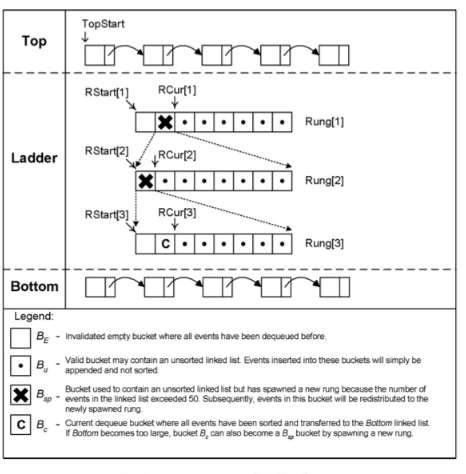
\includegraphics[width=\linewidth]{images/LadderQueue1.png}
\centerline{(a) Structure} \\

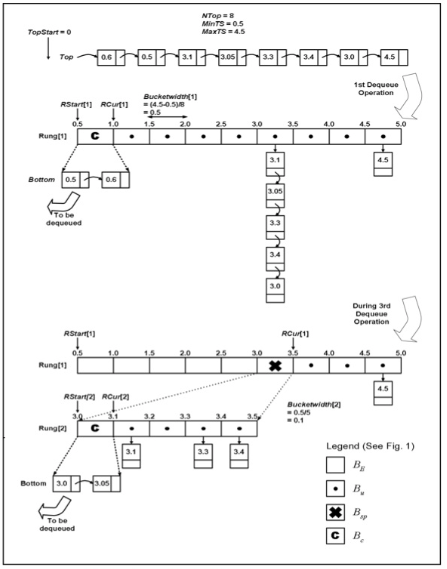
\includegraphics[width=\linewidth]{images/LadderQueue2.png}
\centerline{(b) Dequeue Operations}
\end{minipage}
\textbf{\caption{Structure of Ladder Queue} Source: Tang et al.~\cite{tang-05}}\label{fig:ladderQ}
\end{figure}


\section{Distinguishing aspects of this research}

Our research focuses on distributed memory platforms in which each
parallel process is single threaded. Consequently, our implementation
does not involve thread synchronization issues. However, our 2-tier
design has the ability to further reduce lock contention issues in
multithreaded environments and could provide further performance
boost. To the best of our knowledge, the Fibonnacci heap
(\textbf{fibHeap}) and our 3-tier Heap (\textbf{3tHeap}) are unique
data structures that have potential to be effective in simulations
with high concurrency.

Since it has been established that the Ladder Queue (ladderQ)
outperforms other data structures, we aim to use it for empirical
assessment of our proposed data structures.  However, in contrast to
earlier work, rather than using a linked list based implementation, we
propose an alternative implementation using dynamically growing
arrays, that is, std::vector from the C(++) library. Furthermore, we
trigger \textit{Bottom} to \textit{Ladder} re-bucketing only if the
\textit{Bottom} has events at different timestamps to reduce
inefficiencies. Our 2-tier Ladder Queue (\textbf{2tLadderQ}) is a
novel enhancement to the Ladder Queue to enable its efficient use in
optimistic parallel simulations.
